\documentclass[a4paper,11pt]{article}

\usepackage[english]{babel}
\usepackage{mathrsfs, amssymb, amsmath, amsthm, enumerate}
\usepackage{verbatim,graphicx,geometry,bbm}
%\usetikzlibrary{arrows}
\usepackage[utf8]{inputenc}
\usepackage{authblk}
\usepackage[round]{natbib}
\bibliographystyle{plainnat}

\usepackage{hyperref}

\makeatletter
\def\@biblabel#1{\hspace*{-\labelsep}}
\makeatother
\geometry{left=1in,right=1
in,top=1in,bottom=1in}
\newdimen\dummy
\dummy=\oddsidemargin
\addtolength{\dummy}{72pt}
\marginparwidth=.5\dummy
\marginparsep=.1\dummy


\newcommand{\E}{\mathbb{E}}
\newcommand{\Var}{\mathrm{Var}}
\newcommand{\plim}{\overset{p}{\longrightarrow}}
\newcommand{\dlim}{\overset{d}{\longrightarrow}}

\begin{document}

\section*{Summary of results}

\begin{itemize}
\item The new technology subsidy has positive welfare effects, but it is very low. It was also chosen because of that -- most subsidy values give negative welfare effects. To compare, I used the same subsidy for new technologies. The welfare effect is also positive and much higher, but still very small in percentage terms. There are other new combination subsidy values that yield much better results.

\item Most of the figures are intuitive, and changes happen in the expected direction. One important conclusion is that the cost of inventors does not increase immediately after the subsidy is implemented, which means that the subsidy is not changing too much the configuration of patents that are produced. In fact, the subsidy for new technologies decreases the average amount of technologies produced each year: it creates incentives for inventors in cold product lines to create new technologies, therefore increasing the number of hot product lines -- and inventors in hot product lines are much more likely to do new combinations. This is not true for other values of the subsidy, though.

\item Note also that most of the action is going on because the number of new combinations increases after we subsidize both new combinations \textit{or} new technologies. It just seems that having ideas for new technologies is a very rare event, so its hard to induce any big change by subsidizing this type of patent.
\end{itemize}


\section*{7\% subsidy on new technologies for 50 years}

\begin{itemize}
\item Figures 1 and 2 show how aggregate variables move with the introduction of a subsidy. Figure 1 shows the whole period, while Figure 2 shows only the years after the introduction of the subsidy.
\item Figure 3 expands upon this and shows the difference between the value of these aggregate variables with the subsidy and without the subsidy.
\item Figure 4 and 5 mimic figures 1 and 2 for shares of each type of patent and the number of new technologies produced each year.
\end{itemize}

\begin{figure}[h!]
\centering
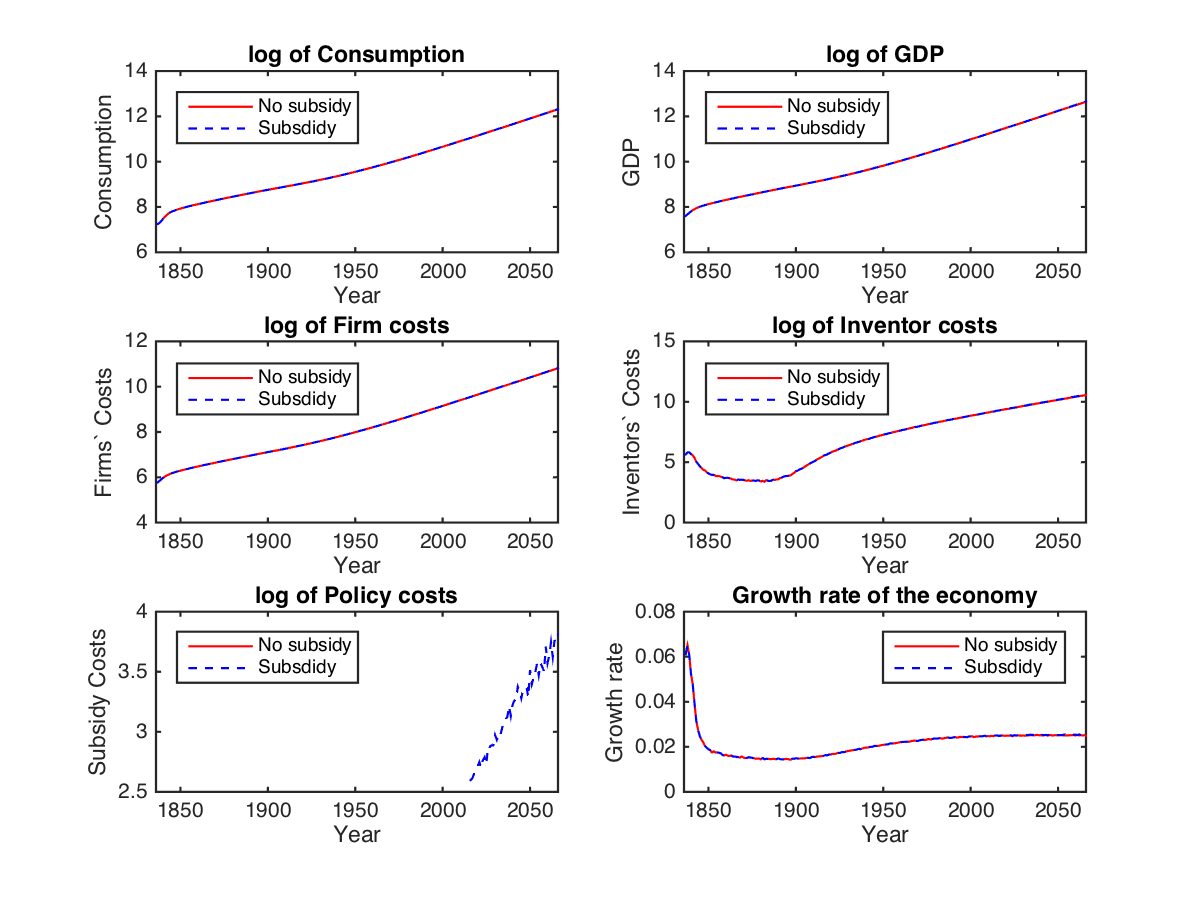
\includegraphics[scale=.6]{figures/aggregatesNT}
\caption{Log of aggregate variables over the whole time span.}
\end{figure}

\begin{figure}[h!]
\centering
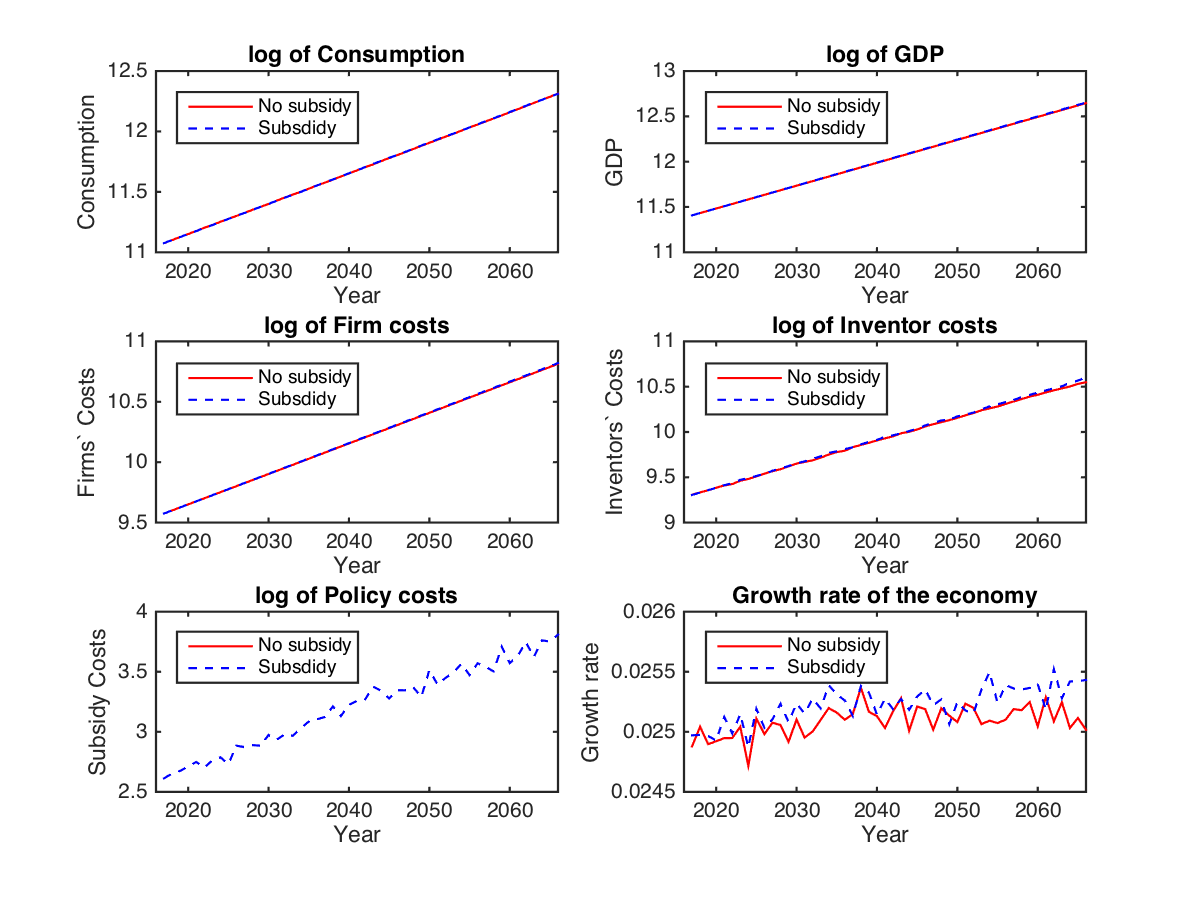
\includegraphics[scale=.6]{figures/aggregates2016NT}
\caption{Log of aggregate variables starting in 2016.}
\end{figure}

\begin{figure}[h!]
\centering
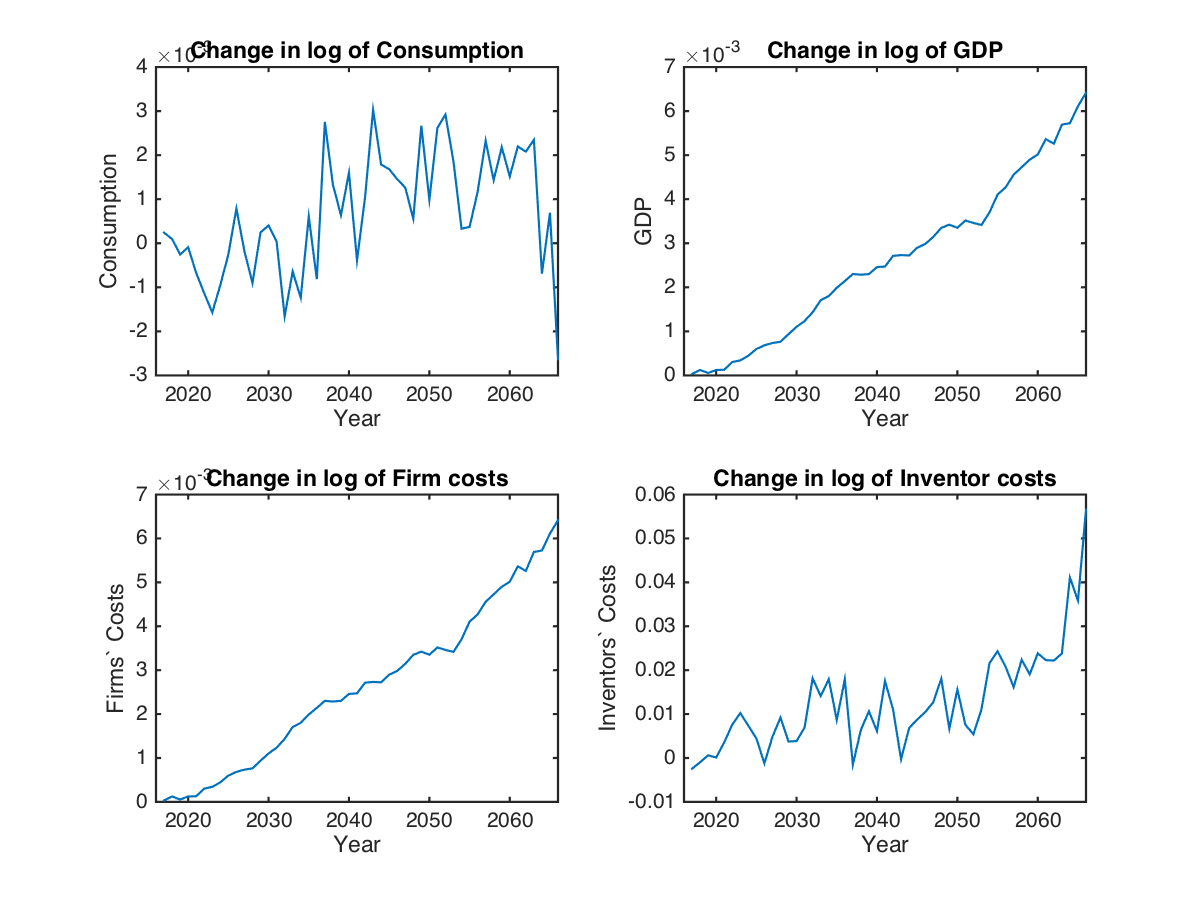
\includegraphics[scale=.6]{figures/aggregates2016_diffNT}
\caption{Difference between values with subsidy and without subsidy.}
\end{figure}

\begin{figure}[h!]
\centering
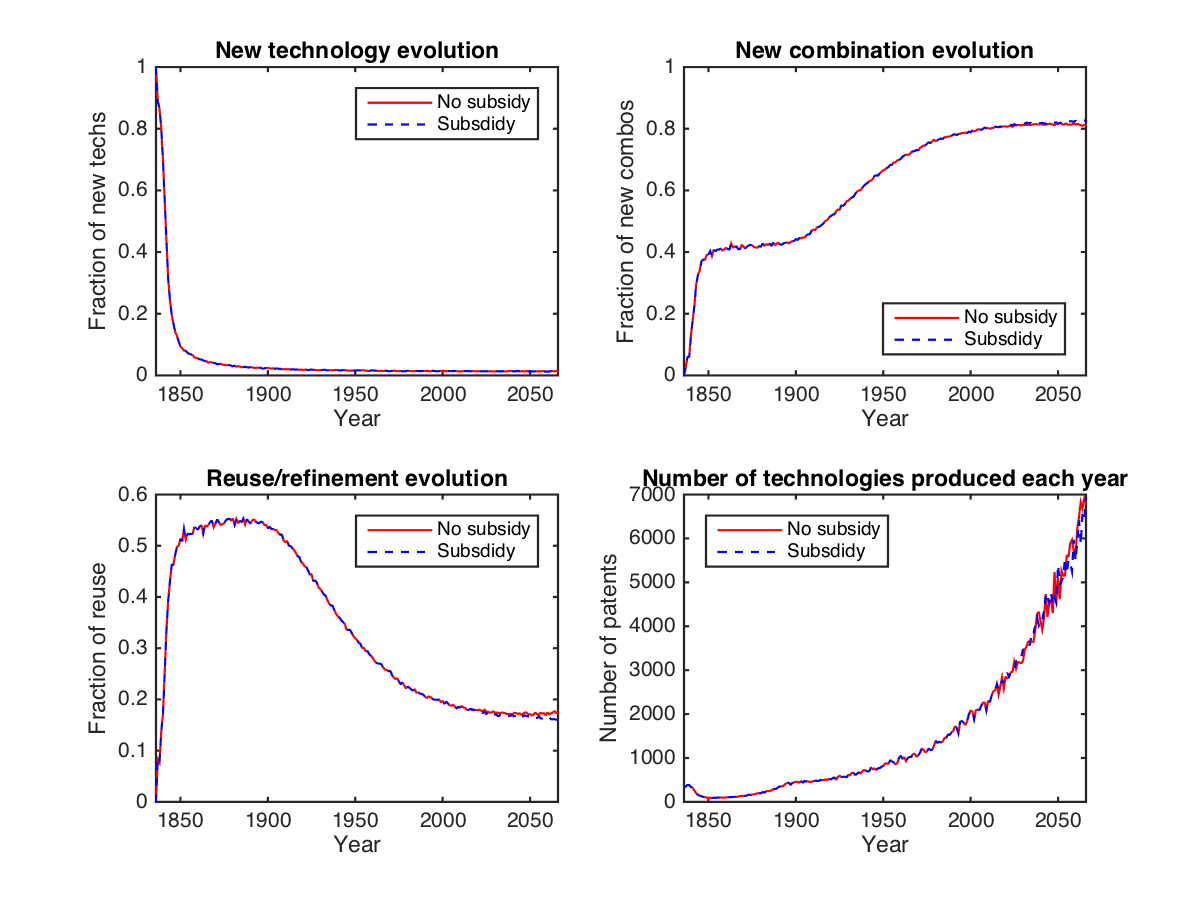
\includegraphics[scale=.6]{figures/patentsNT}
\caption{Evolution of patent type fractions, whole time period.}
\end{figure}

\begin{figure}[h!]
\centering
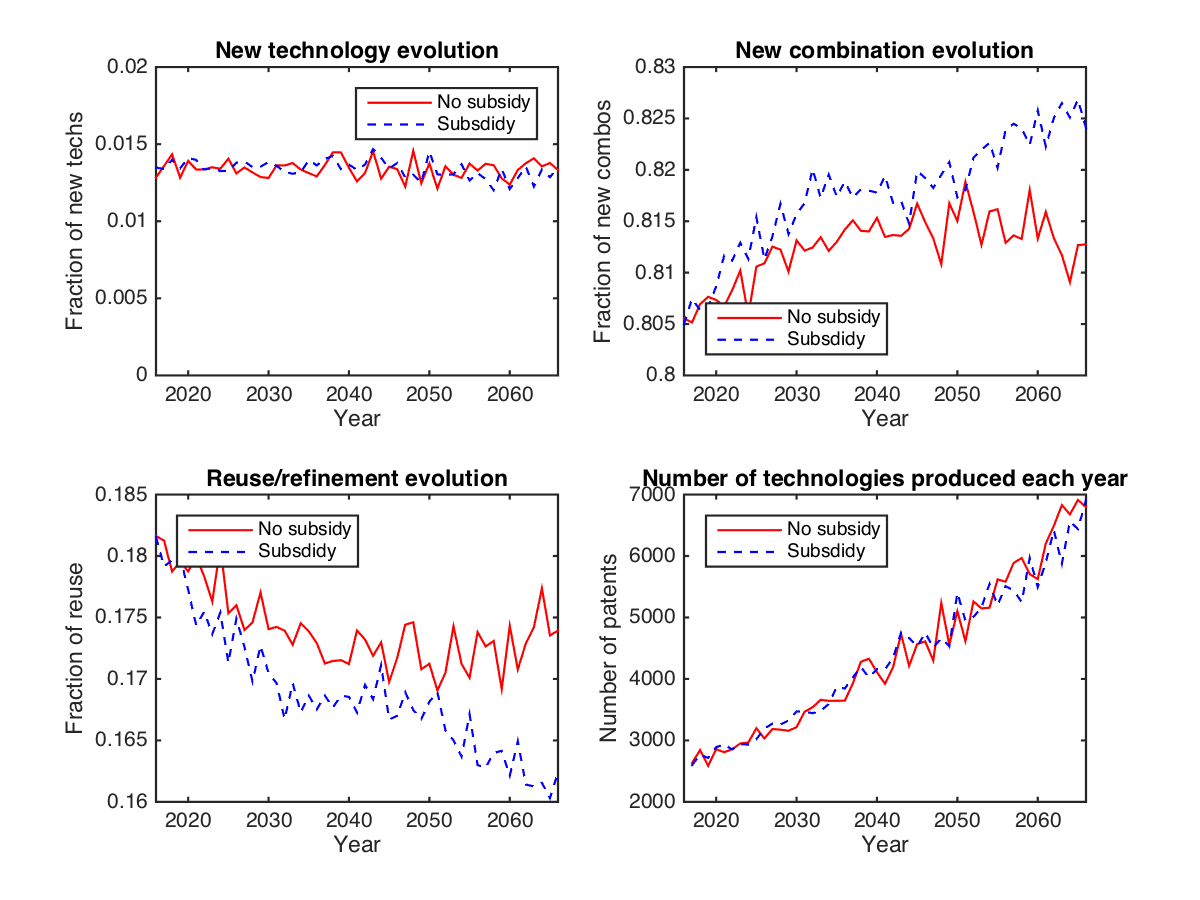
\includegraphics[scale=.6]{figures/patents2016NT}
\caption{Evolution of patent type fractions, starting in 2016.}
\end{figure}

\clearpage

\section*{7\% subsidy on new combinations over 50 years.}

\begin{figure}[h!]
\centering
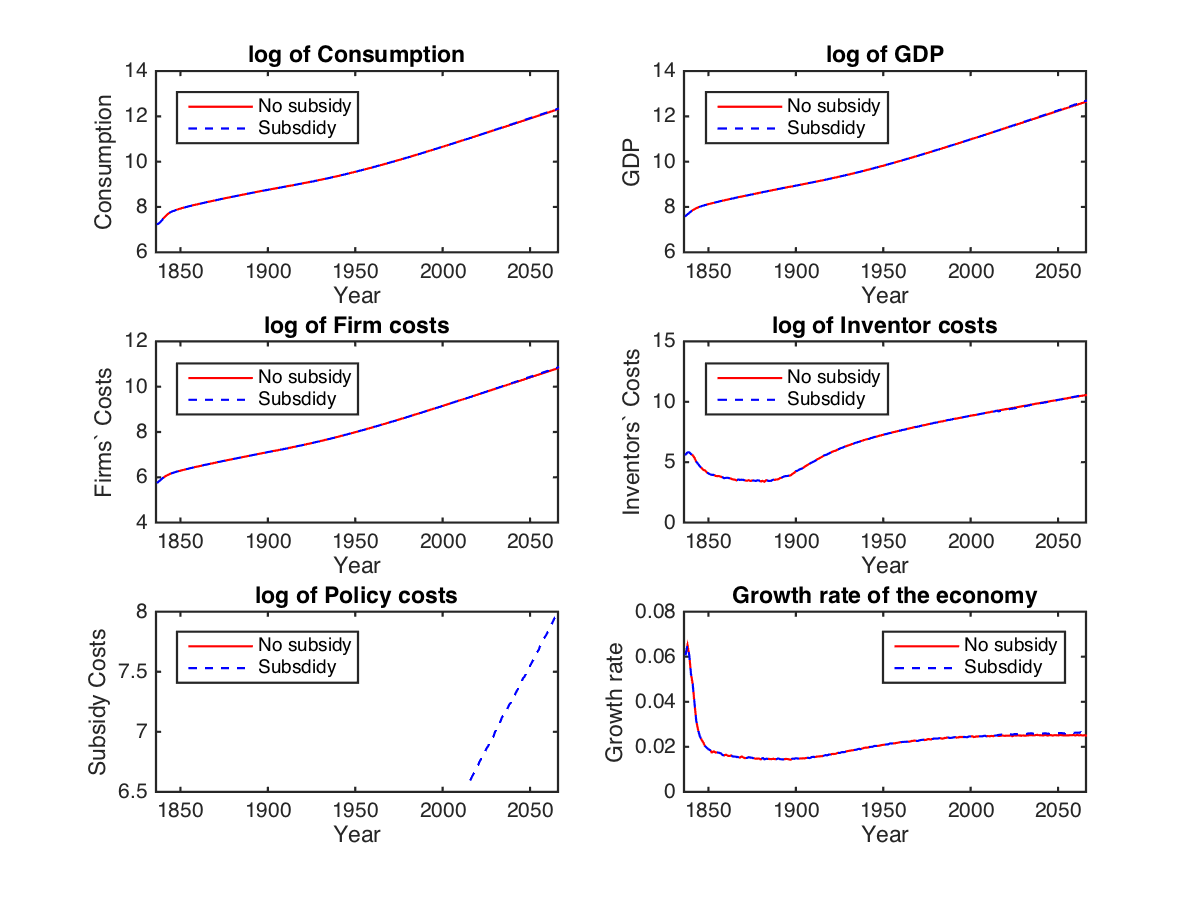
\includegraphics[scale=.6]{figures/aggregatesNC}
\caption{Log of aggregate variables over the whole time span.}
\end{figure}

\begin{figure}[h!]
\centering
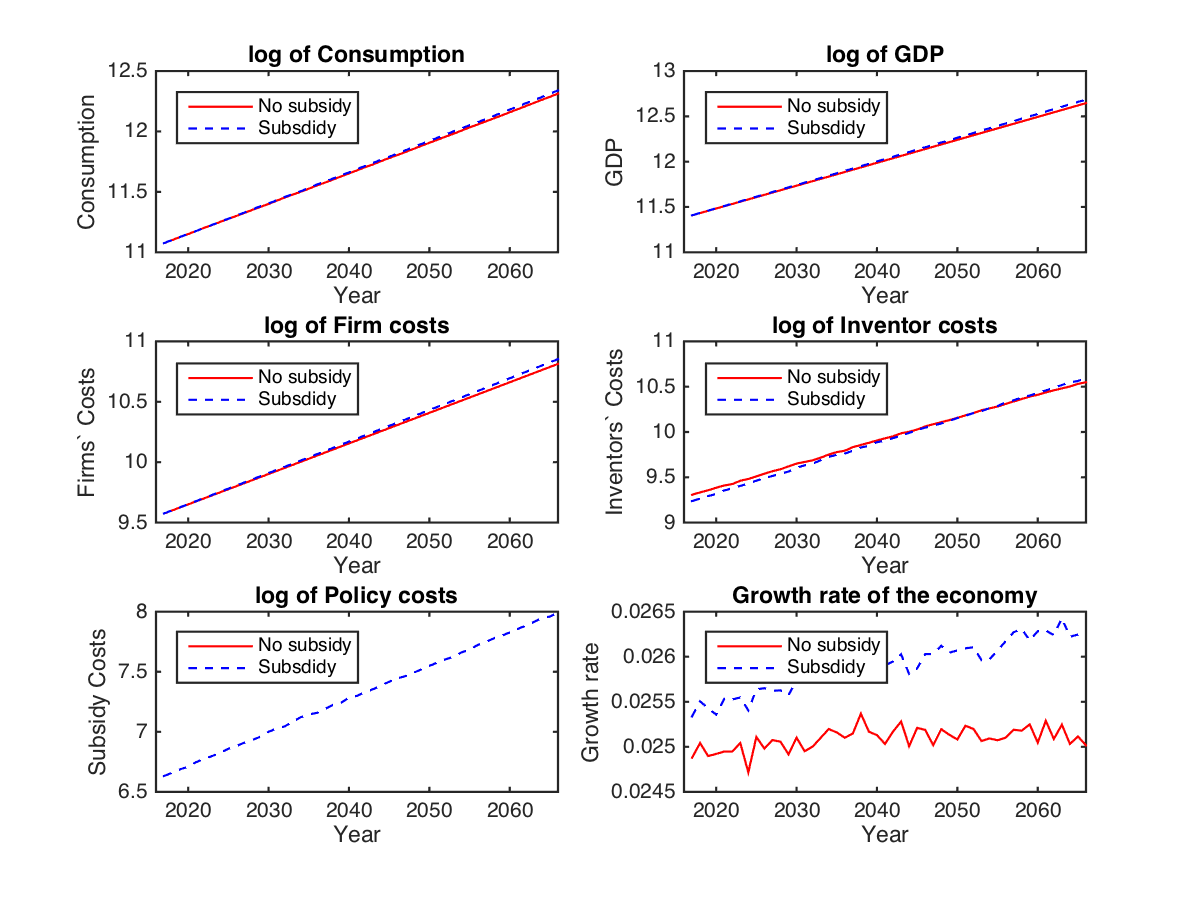
\includegraphics[scale=.6]{figures/aggregates2016NC}
\caption{Log of aggregate variables starting in 2016.}
\end{figure}

\begin{figure}[h!]
\centering
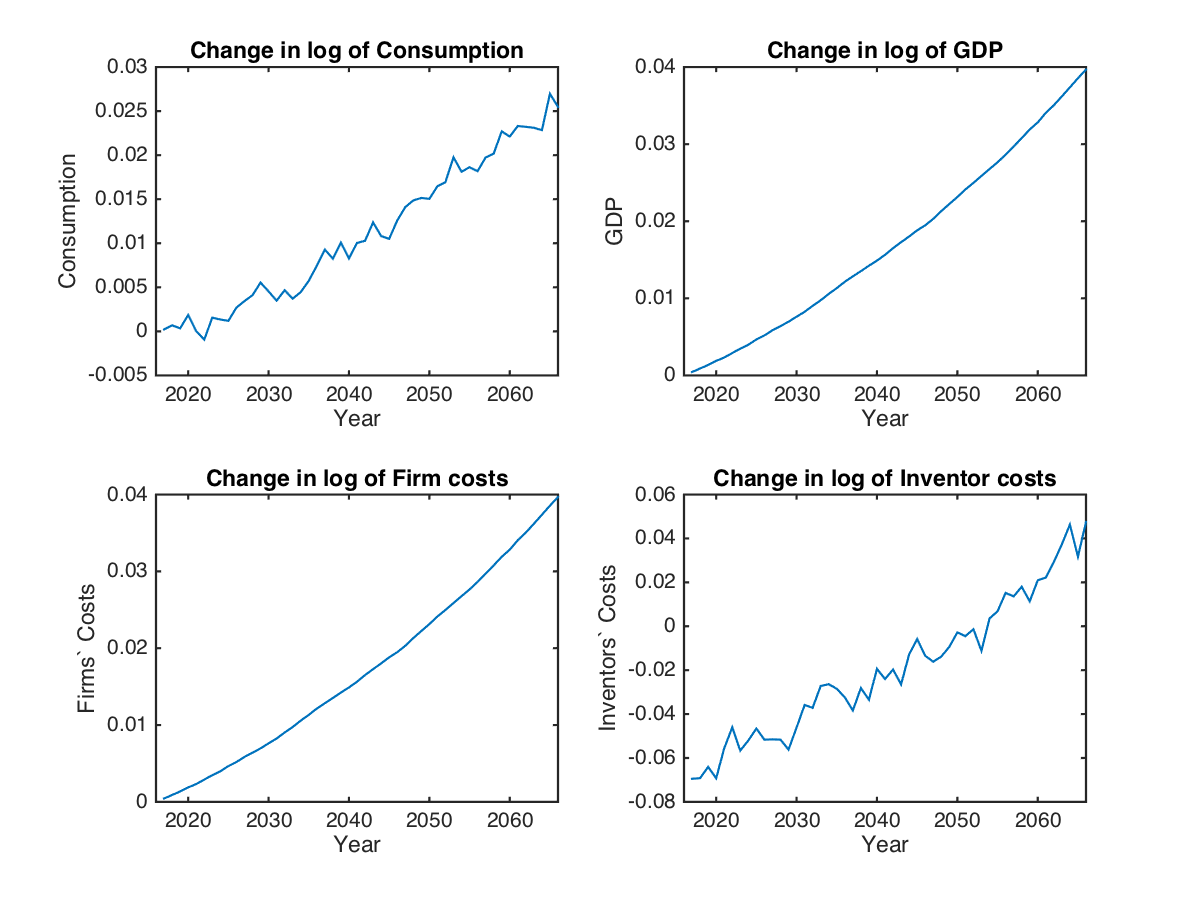
\includegraphics[scale=.6]{figures/aggregates2016_diffNC}
\caption{Difference between values with subsidy and without subsidy.}
\end{figure}

\begin{figure}[h!]
\centering
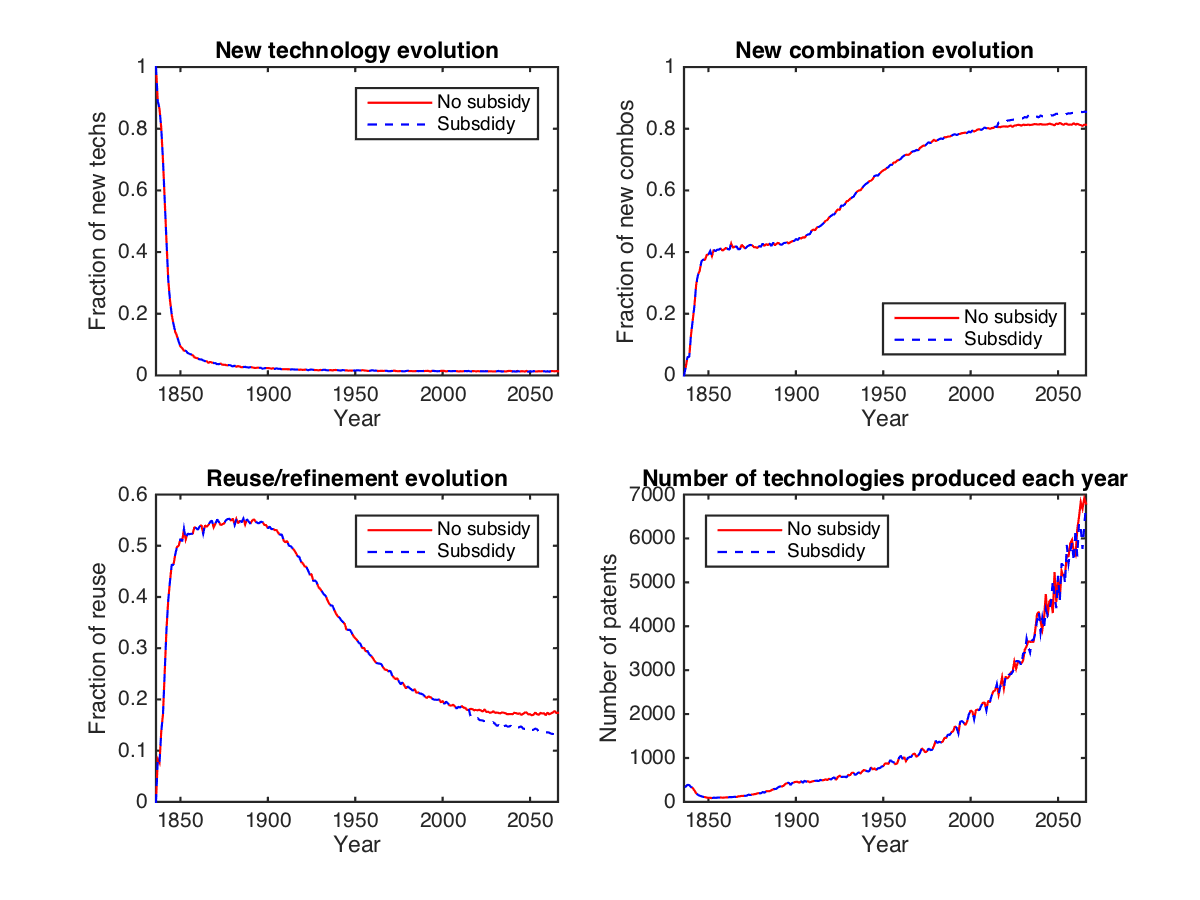
\includegraphics[scale=.6]{figures/patentsNC}
\caption{Evolution of patent type fractions, whole time period.}
\end{figure}

\begin{figure}[h!]
\centering
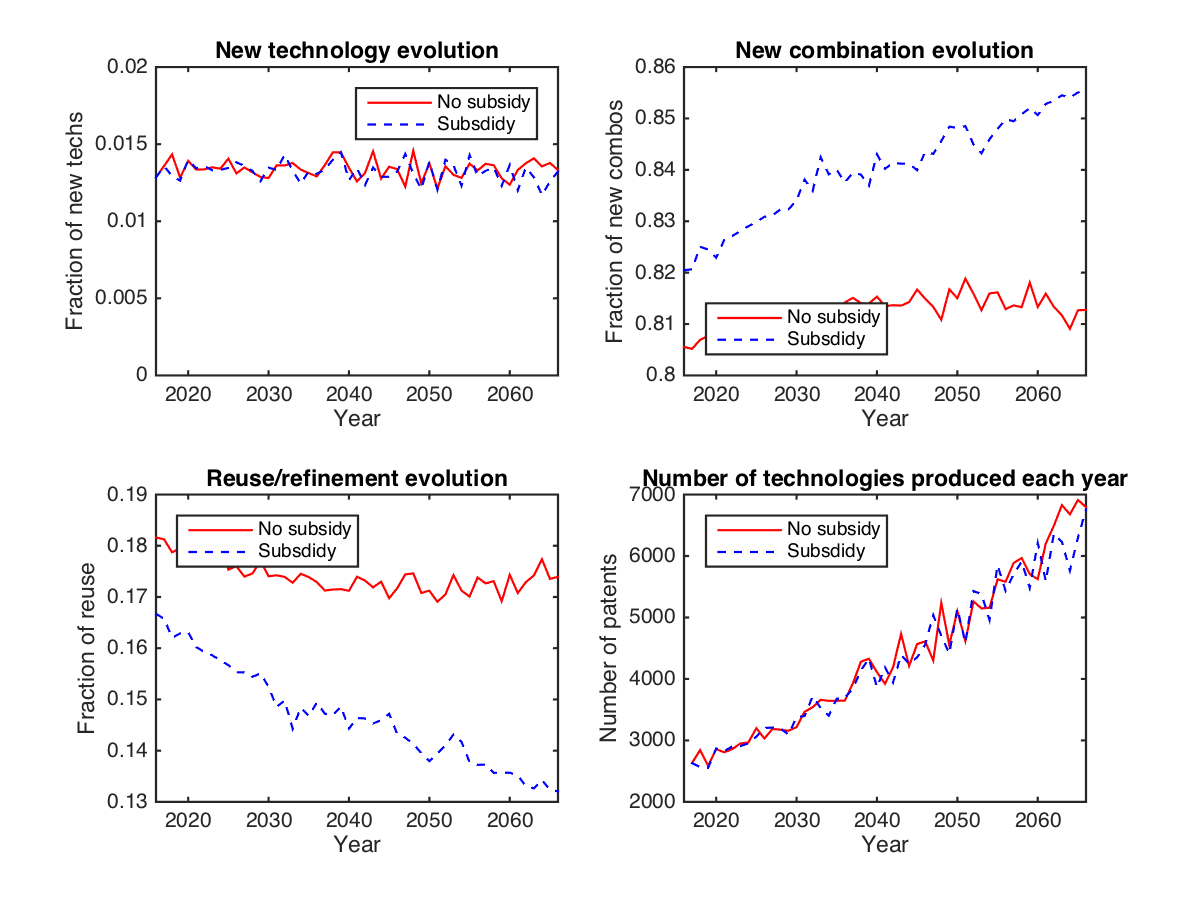
\includegraphics[scale=.6]{figures/patents2016NC}
\caption{Evolution of patent type fractions, starting in 2016.}
\end{figure}

\end{document}